\section{Widgets (3)}\label{widgets-3}

\subsection{Open signal}\label{open-signal}

\subsubsection{G\_APPLICATION\_HANDLES\_OPEN
flag}\label{g_application_handles_open-flag}

We made a very simple editor in the previous section with GtkTextView,
GtkTextBuffer and GtkScrolledWindow. We will add file-read ability to
the program and improve it to a file viewer.

The easiest way to give a filename is to use a command line argument.

\begin{lstlisting}
$ ./a.out filename
\end{lstlisting}

The program will open the file and insert its contents into the
GtkTextBuffer.

To do this, we need to know how GtkApplication (or GApplication)
recognizes arguments. This is described in the
\href{https://docs.gtk.org/gio/class.Application.html}{GIO API Reference
-- Application}.

When GtkApplication is created, a flag (GApplicationFlags) is given as
an argument.

\begin{lstlisting}[language=C]
GtkApplication *
gtk_application_new (const gchar *application_id, GApplicationFlags flags);
\end{lstlisting}

This tutorial explains only two flags,
\passthrough{\lstinline!G\_APPLICATION\_DEFAULT\_FLAGS!} and
\passthrough{\lstinline!G\_APPLICATION\_HANDLES\_OPEN!}.

\passthrough{\lstinline!G\_APPLICATION\_FLAGS\_NONE!} was used instead
of \passthrough{\lstinline!G\_APPLICATION\_DEFAULT\_FLAGS!} before GIO
version2.73.3 (GLib 2.73.3 5/Aug/2022). Now it is deprecated and
\passthrough{\lstinline!G\_APPLICATION\_DEFAULT\_FLAGS!} is recommended.

For further information, see
\href{https://docs.gtk.org/gio/flags.ApplicationFlags.html}{GIO API
Reference -- ApplicationFlags} and
\href{https://docs.gtk.org/gio/method.Application.run.html}{GIO API
Reference -- g\_application\_run}.

We've already used
\passthrough{\lstinline!G\_APPLICATION\_DEFAULT\_FLAGS!}, as it is the
simplest option, and no command line arguments are allowed. If you give
arguments, an error will occur.

The flag \passthrough{\lstinline!G\_APPLICATION\_HANDLES\_OPEN!} is the
second simplest option. It allows arguments but only filenames.

\begin{lstlisting}[language=C]
app = gtk_application_new ("com.github.ToshioCP.tfv3", G_APPLICATION_HANDLES_OPEN);
\end{lstlisting}

\subsubsection{open signal}\label{open-signal-1}

When \passthrough{\lstinline!G\_APPLICATION\_HANDLES\_OPEN!} flag is
given to the application, two signals are available.

\begin{itemize}
\tightlist
\item
  activate signal: This signal is emitted when there's no argument.
\item
  open signal: This signal is emitted when there is at least one
  argument.
\end{itemize}

The handler of the ``open'' signal is defined as follows.

\begin{lstlisting}[language=C]
void
open (
  GApplication* self,
  gpointer files,
  gint n_files,
  gchar* hint,
  gpointer user_data
)
\end{lstlisting}

The parameters are:

\begin{itemize}
\tightlist
\item
  self: the application instance (usually GtkApplication)
\item
  files: an array of GFiles. {[}array length=n\_files{]} {[}element-type
  GFile{]}
\item
  n\_files: the number of the elements of
  \passthrough{\lstinline!files!}
\item
  hint: a hint provided by the calling instance (usually it can be
  ignored)
\item
  user\_data: user data that is set when the signal handler was
  connected.
\end{itemize}

\subsection{File viewer}\label{file-viewer}

\subsubsection{What is a file viewer?}\label{what-is-a-file-viewer}

A file viewer is a program that displays text files. Our file viewer is
as follows.

\begin{itemize}
\tightlist
\item
  When arguments are given, it recognizes the first argument as a
  filename and opens it.
\item
  The second argument and after are ignored.
\item
  If there's no argument, it shows an error message and quit.
\item
  If it successfully opens the file, it reads the contents of the file,
  inserts them to GtkTextBuffer and shows the window.
\item
  If it fails to open the file, it shows an error message and quit.
\end{itemize}

The program is shown below.

\begin{lstlisting}[language=C, numbers=left]
#include <gtk/gtk.h>

static void
app_activate (GApplication *app) {
  g_printerr ("You need a filename argument.\n");
}

static void
app_open (GApplication *app, GFile ** files, int n_files, char *hint) {
  GtkWidget *win;
  GtkWidget *scr;
  GtkWidget *tv;
  GtkTextBuffer *tb;
  char *contents;
  gsize length;
  char *filename;
  GError *err = NULL;

  win = gtk_application_window_new (GTK_APPLICATION (app));
  gtk_window_set_default_size (GTK_WINDOW (win), 400, 300);

  scr = gtk_scrolled_window_new ();
  gtk_window_set_child (GTK_WINDOW (win), scr);

  tv = gtk_text_view_new ();
  tb = gtk_text_view_get_buffer (GTK_TEXT_VIEW (tv));
  gtk_text_view_set_wrap_mode (GTK_TEXT_VIEW (tv), GTK_WRAP_WORD_CHAR);
  gtk_text_view_set_editable (GTK_TEXT_VIEW (tv), FALSE);
  gtk_scrolled_window_set_child (GTK_SCROLLED_WINDOW (scr), tv);

  if (g_file_load_contents (files[0], NULL, &contents, &length, NULL, &err)) {
    gtk_text_buffer_set_text (tb, contents, length);
    g_free (contents);
    if ((filename = g_file_get_basename (files[0])) != NULL) {
      gtk_window_set_title (GTK_WINDOW (win), filename);
      g_free (filename);
    }
    gtk_window_present (GTK_WINDOW (win));
  } else {
    g_printerr ("%s.\n", err->message);
    g_error_free (err);
    gtk_window_destroy (GTK_WINDOW (win));
  }
}

int
main (int argc, char **argv) {
  GtkApplication *app;
  int stat;

  app = gtk_application_new ("com.github.ToshioCP.tfv3", G_APPLICATION_HANDLES_OPEN);
  g_signal_connect (app, "activate", G_CALLBACK (app_activate), NULL);
  g_signal_connect (app, "open", G_CALLBACK (app_open), NULL);
  stat = g_application_run (G_APPLICATION (app), argc, argv);
  g_object_unref (app);
  return stat;
}
\end{lstlisting}

Save it as \passthrough{\lstinline!tfv3.c!}. If you've downloaded this
repository, the file is \passthrough{\lstinline!src/tfv/tfv3.c!}.
Compile and run it.

\begin{lstlisting}
$ comp tfv3
$ ./a.out tfv3.c
\end{lstlisting}

\begin{figure}
\centering
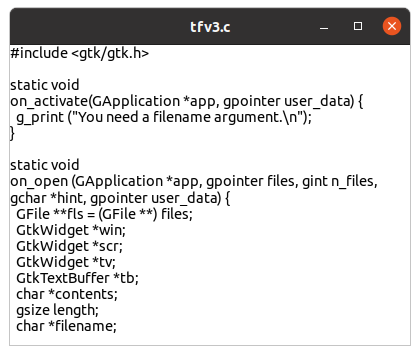
\includegraphics[width=6.3cm,height=5.325cm]{../image/screenshot_tfv3.png}
\caption{File viewer}
\end{figure}

The function \passthrough{\lstinline!main!} has only two changes from
the previous version.

\begin{itemize}
\tightlist
\item
  \passthrough{\lstinline!G\_APPLICATION\_DEFAULT\_FLAGS!} is replaced
  by \passthrough{\lstinline!G\_APPLICATION\_HANDLES\_OPEN!}
\item
  \passthrough{\lstinline!g\_signal\_connect (app, "open", G\_CALLBACK (app\_open), NULL)!}
  is added.
\end{itemize}

When the flag \passthrough{\lstinline!G\_APPLICATION\_HANDLES\_OPEN!} is
given to \passthrough{\lstinline!gtk\_application\_new!} function, the
application behaves like this:

\begin{itemize}
\tightlist
\item
  If the application is run without command line arguments, it emits
  ``activate'' signal when it is activated.
\item
  If the application is run with command line arguments, it emits
  ``open'' signal when it is activated.
\end{itemize}

The handler \passthrough{\lstinline!app\_activate!} becomes very simple.
It just outputs an error message and returns to the caller. Then the
application quits immediately because no window is created.

The main work is done in the handler
\passthrough{\lstinline!app\_open!}.

\begin{itemize}
\tightlist
\item
  Creates GtkApplicationWindow, GtkScrolledWindow, GtkTextView and
  GtkTextBuffer and connects them together
\item
  Sets wrap mode to \passthrough{\lstinline!GTK\_WRAP\_WORD\_CHAR!} in
  GtktextView
\item
  Sets GtkTextView to non-editable because the program isn't an editor
  but only a viewer
\item
  Reads the file and inserts the text into GtkTextBuffer (this will be
  explained later)
\item
  If the file is not opened, outputs an error message and destroys the
  window. This makes the application quit.
\end{itemize}

The following is the file reading part of the program.

\begin{lstlisting}[language=C]
if (g_file_load_contents (files[0], NULL, &contents, &length, NULL, &err)) {
  gtk_text_buffer_set_text (tb, contents, length);
  g_free (contents);
  if ((filename = g_file_get_basename (files[0])) != NULL) {
    gtk_window_set_title (GTK_WINDOW (win), filename);
    g_free (filename);
  }
  gtk_window_present (GTK_WINDOW (win));
} else {
  g_printerr ("%s.\n", err->message);
  g_error_free (err);
  gtk_window_destroy (GTK_WINDOW (win));
}
\end{lstlisting}

The function \passthrough{\lstinline!g\_file\_load\_contents!} loads the
file contents into a temporary buffer, which is automatically allocated
and sets \passthrough{\lstinline!contents!} to point the buffer. The
length of the buffer is assigned to \passthrough{\lstinline!length!}. It
returns \passthrough{\lstinline!TRUE!} if the file's contents are
successfully loaded. If an error occurs, it returns
\passthrough{\lstinline!FALSE!} and sets the variable
\passthrough{\lstinline!err!} to point a newly created GError structure.
The caller takes ownership of the GError structure and is responsible
for freeing it. If you want to know the details about
g\_file\_load\_contents, see
\href{https://docs.gtk.org/gio/method.File.load_contents.html}{g file
load contents}.

If it has successfully read the file, it inserts the contents into
GtkTextBuffer, frees the temporary buffer pointed by
\passthrough{\lstinline!contents!}, sets the title of the window, frees
the memories pointed by \passthrough{\lstinline!filename!} and then
shows the window.

If it fails, \passthrough{\lstinline!g\_file\_load\_contents!} sets
\passthrough{\lstinline!err!} to point a newly created GError structure.
The structure is:

\begin{lstlisting}[language=C]
struct GError {
  GQuark domain;
  int code;
  char* message;
}
\end{lstlisting}

The \passthrough{\lstinline!message!} member is used most often. It
points an error message. A function
\passthrough{\lstinline!g\_error\_free!} is used to free the memory of
the structure. See
\href{https://docs.gtk.org/glib/struct.Error.html}{GError}.

The program above outputs an error message, frees
\passthrough{\lstinline!err!} and destroys the window and finally make
the program quit.

\subsection{GtkNotebook}\label{gtknotebook}

GtkNotebook is a container widget that contains multiple widgets with
tabs. It shows only one child at a time. Another child will be shown
when its tab is clicked.

\begin{figure}
\centering
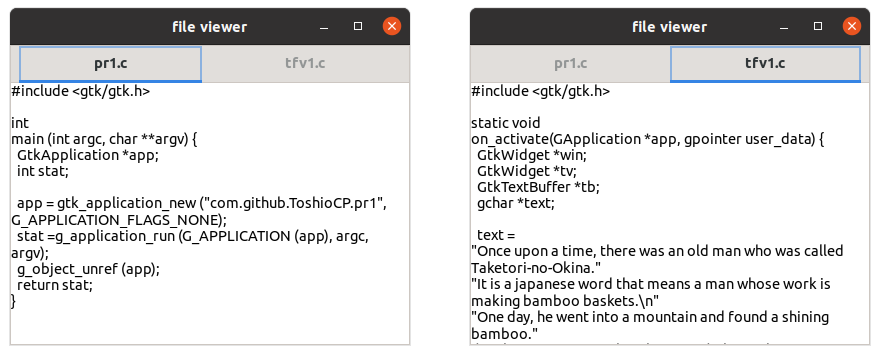
\includegraphics[width=13.2cm,height=5.325cm]{../image/screenshot_gtk_notebook.png}
\caption{GtkNotebook}
\end{figure}

The left image is the window at the startup. The file
\passthrough{\lstinline!pr1.c!} is shown and its filename is in the left
tab. After clicking on the right tab, the contents of the file
\passthrough{\lstinline!tfv1.c!} is shown (the right image).

The following is \passthrough{\lstinline!tfv4.c!}. It has GtkNoteBook
widget. It is inserted as a child of GtkApplicationWindow and contains
multiple GtkScrolledWindow.

\begin{lstlisting}[language=C, numbers=left]
#include <gtk/gtk.h>

static void
app_activate (GApplication *app) {
  g_printerr ("You need filename arguments.\n");
}

static void
app_open (GApplication *app, GFile ** files, gint n_files, gchar *hint) {
  GtkWidget *win;
  GtkWidget *nb;
  GtkWidget *lab;
  GtkNotebookPage *nbp;
  GtkWidget *scr;
  GtkWidget *tv;
  GtkTextBuffer *tb;
  char *contents;
  gsize length;
  char *filename;
  int i;
  GError *err = NULL;

  win = gtk_application_window_new (GTK_APPLICATION (app));
  gtk_window_set_title (GTK_WINDOW (win), "file viewer");
  gtk_window_set_default_size (GTK_WINDOW (win), 600, 400);
  nb = gtk_notebook_new ();
  gtk_window_set_child (GTK_WINDOW (win), nb);

  for (i = 0; i < n_files; i++) {
    if (g_file_load_contents (files[i], NULL, &contents, &length, NULL, &err)) {
      scr = gtk_scrolled_window_new ();
      tv = gtk_text_view_new ();
      tb = gtk_text_view_get_buffer (GTK_TEXT_VIEW (tv));
      gtk_text_view_set_wrap_mode (GTK_TEXT_VIEW (tv), GTK_WRAP_WORD_CHAR);
      gtk_text_view_set_editable (GTK_TEXT_VIEW (tv), FALSE);
      gtk_scrolled_window_set_child (GTK_SCROLLED_WINDOW (scr), tv);

      gtk_text_buffer_set_text (tb, contents, length);
      g_free (contents);
      if ((filename = g_file_get_basename (files[i])) != NULL) {
        lab = gtk_label_new (filename);
        g_free (filename);
      } else
        lab = gtk_label_new ("");
      gtk_notebook_append_page (GTK_NOTEBOOK (nb), scr, lab);
      nbp = gtk_notebook_get_page (GTK_NOTEBOOK (nb), scr);
      g_object_set (nbp, "tab-expand", TRUE, NULL);
    } else {
      g_printerr ("%s.\n", err->message);
      g_clear_error (&err);
    }
  }
  if (gtk_notebook_get_n_pages (GTK_NOTEBOOK (nb)) > 0)
    gtk_window_present (GTK_WINDOW (win));
  else
    gtk_window_destroy (GTK_WINDOW (win));
}

int
main (int argc, char **argv) {
  GtkApplication *app;
  int stat;

  app = gtk_application_new ("com.github.ToshioCP.tfv4", G_APPLICATION_HANDLES_OPEN);
  g_signal_connect (app, "activate", G_CALLBACK (app_activate), NULL);
  g_signal_connect (app, "open", G_CALLBACK (app_open), NULL);
  stat = g_application_run (G_APPLICATION (app), argc, argv);
  g_object_unref (app);
  return stat;
}
\end{lstlisting}

Most of the changes are in the function
\passthrough{\lstinline!app\_open!}. The numbers at the left of the
following items are line numbers in the source code.

\begin{itemize}
\tightlist
\item
  11-13: Variables \passthrough{\lstinline!nb!},
  \passthrough{\lstinline!lab!} and \passthrough{\lstinline!nbp!} are
  defined. They point GtkNotebook, GtkLabel and GtkNotebookPage
  respectively.
\item
  24: The window's title is set to ``file viewer''.
\item
  25: The default size of the window is 600x400.
\item
  26-27: GtkNotebook is created and inserted to the GtkApplicationWindow
  as a child.
\item
  29-57: For-loop. The variable \passthrough{\lstinline!files[i]!}
  points i-th GFile, which is created by the GtkApplication from the
  i-th command line argument.
\item
  31-36: GtkScrollledWindow, GtkTextView are created. GtkTextBuffer is
  got from the GtkTextView. The GtkTextView is connected to the
  GtkScrolledWindow as a child.
\item
  38-39: inserts the contents of the file into GtkTextBuffer and frees
  the memory pointed by \passthrough{\lstinline!contents!}.
\item
  40-42: If the filename is taken from the GFile, GtkLabel is created
  with the filename. The string \passthrough{\lstinline!filename!} is
  freed..
\item
  43-44: If it fails to take the filename, empty string GtkLabel is
  created.
\item
  45-46: Appends a GtkScrolledWindow to the GtkNotebook as a child. And
  the GtkLabel is set as the child's tab. At the same time, a
  GtkNoteBookPage is created automatically. The function
  \passthrough{\lstinline!gtk\_notebook\_get\_page!} returns the
  GtkNotebookPage of the child (GtkScrolledWindow).
\item
  47: GtkNotebookPage has ``tab-expand'' property. If it is set to TRUE
  then the tab expands horizontally as long as possible. If it is FALSE,
  then the width of the tab is determined by the size of the label.
  \passthrough{\lstinline!g\_object\_set!} is a general function to set
  properties of objects. See
  \href{https://docs.gtk.org/gobject/method.Object.set.html}{GObject API
  Reference -- g\_object\_set}.
\item
  48-50: If it fails to read the file, the error message is shown. The
  function \passthrough{\lstinline!g\_clear\_error (\&err)!} works like
  \passthrough{\lstinline!g\_error\_free (err); err = NULL!}.
\item
  53-56: If at least one page exists, the window is shown. Otherwise,
  the window is destroyed and the application quits.
\end{itemize}
